\section{Measurements}
\label{sec:measurements}
In order to quantify the performance of the Parallella board and our LSH based KNN search, we measure several parameters such as:
\begin{itemize}
\item Computation time of n\"{a}ive KNN search
\item Computation time of LSH based KNN search
\item Power consumption of Parallella board
\end{itemize}
\subsection{N\"{a}ive KNN Search computation time}
\label{subsec:nknn_comptime}
Since it would have been computationally infeasible to conduct a full KNN (K=$10^6$) search over all the records in the dataset, we selected 256 and 1000 records and conducted a naive KNN search with K=256, 1000 respectively. 
As mentioned in Section \ref{sec:methodology}, we use hamming distance as our distance. We ran the KNN search on a typical laptop (Macbook Air with Intel i7-2677M), high performance desktop (Mac Pro with Intel Xeon E5-1680), and on the Parallella (Epiphany III). Figure \ref{fig:fullK256_1000} shows the comparative performance of these three processors. For 256 record dataset (Figure \ref{fig:k256_comptime}), we see that the Parallella board performs 23.05\% faster than the Macbook Air, but is slower than the Mac Pro by 13\%. For 1000 record dataset (Figure \ref{fig:k1000_comptime}), we see that the Parallella board is faster than the Macbook Air by 30\%, but is slower than the Mac Pro by only 7\%.

\textbf{\underline{Result}}: \textit{Using the Epiphany multicore chip on the Parallella board, for a n\"{a}ive KNN search, we were able to achieve an average speed up of 26.5\% compared to a high end Macbook Air with an Intel i7-2677M processor.}
\begin{figure}
\centering
\begin{subfigure}[b]{0.45\textwidth}
	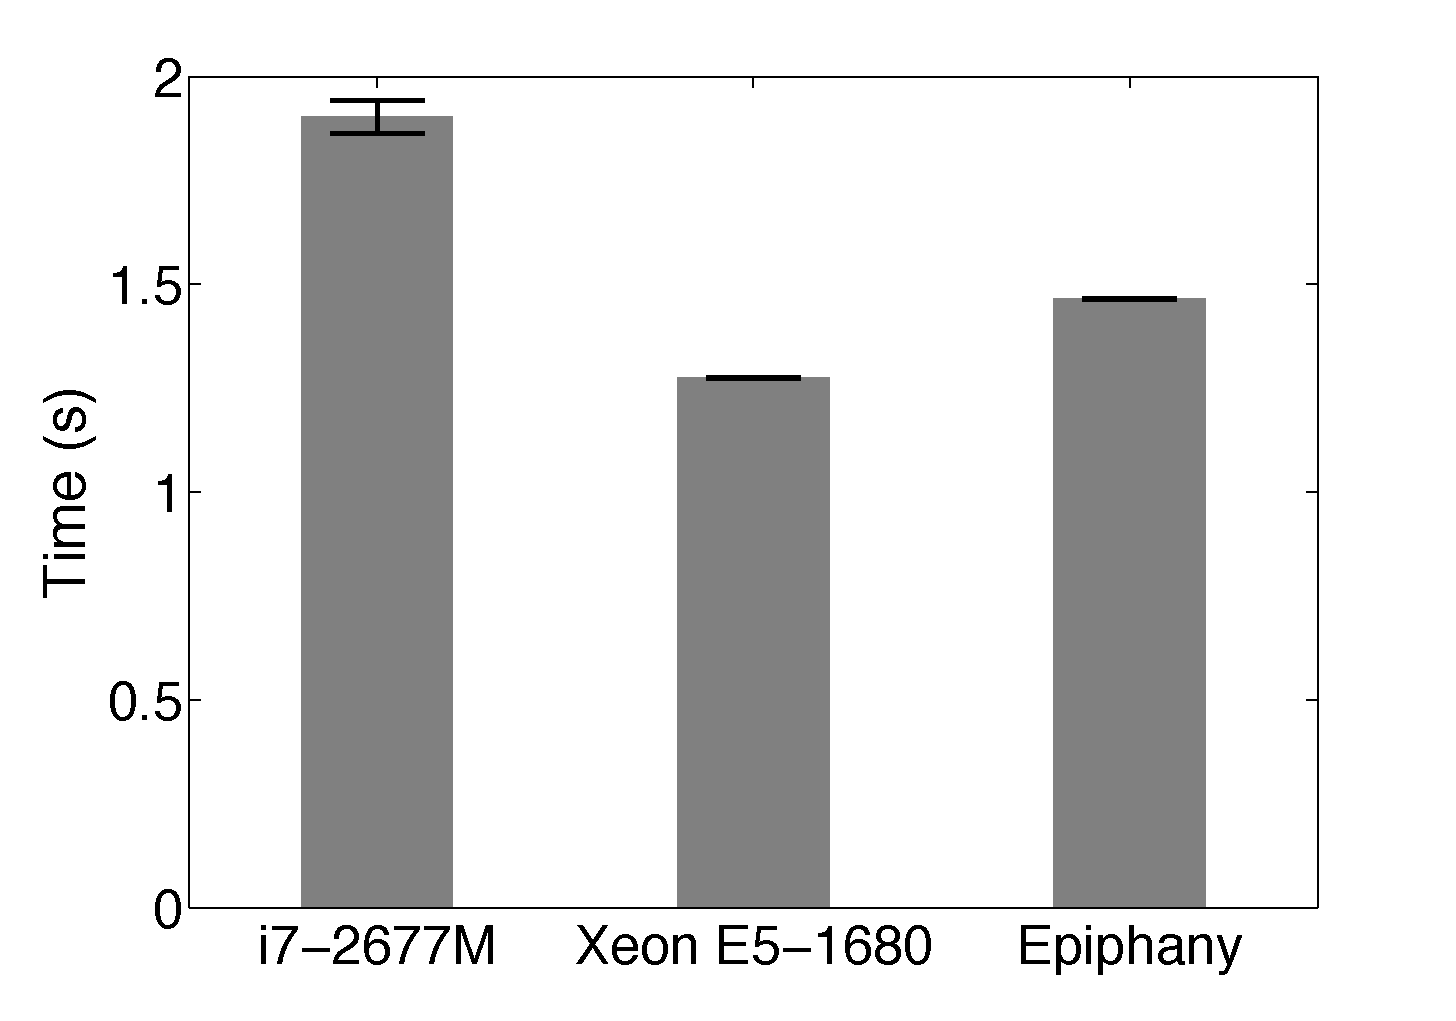
\includegraphics[width=\textwidth]{gt_256.pdf}
	\caption{256 records}
	\label{fig:k256_comptime}
\end{subfigure}
~
\begin{subfigure}[b]{0.45\textwidth}
	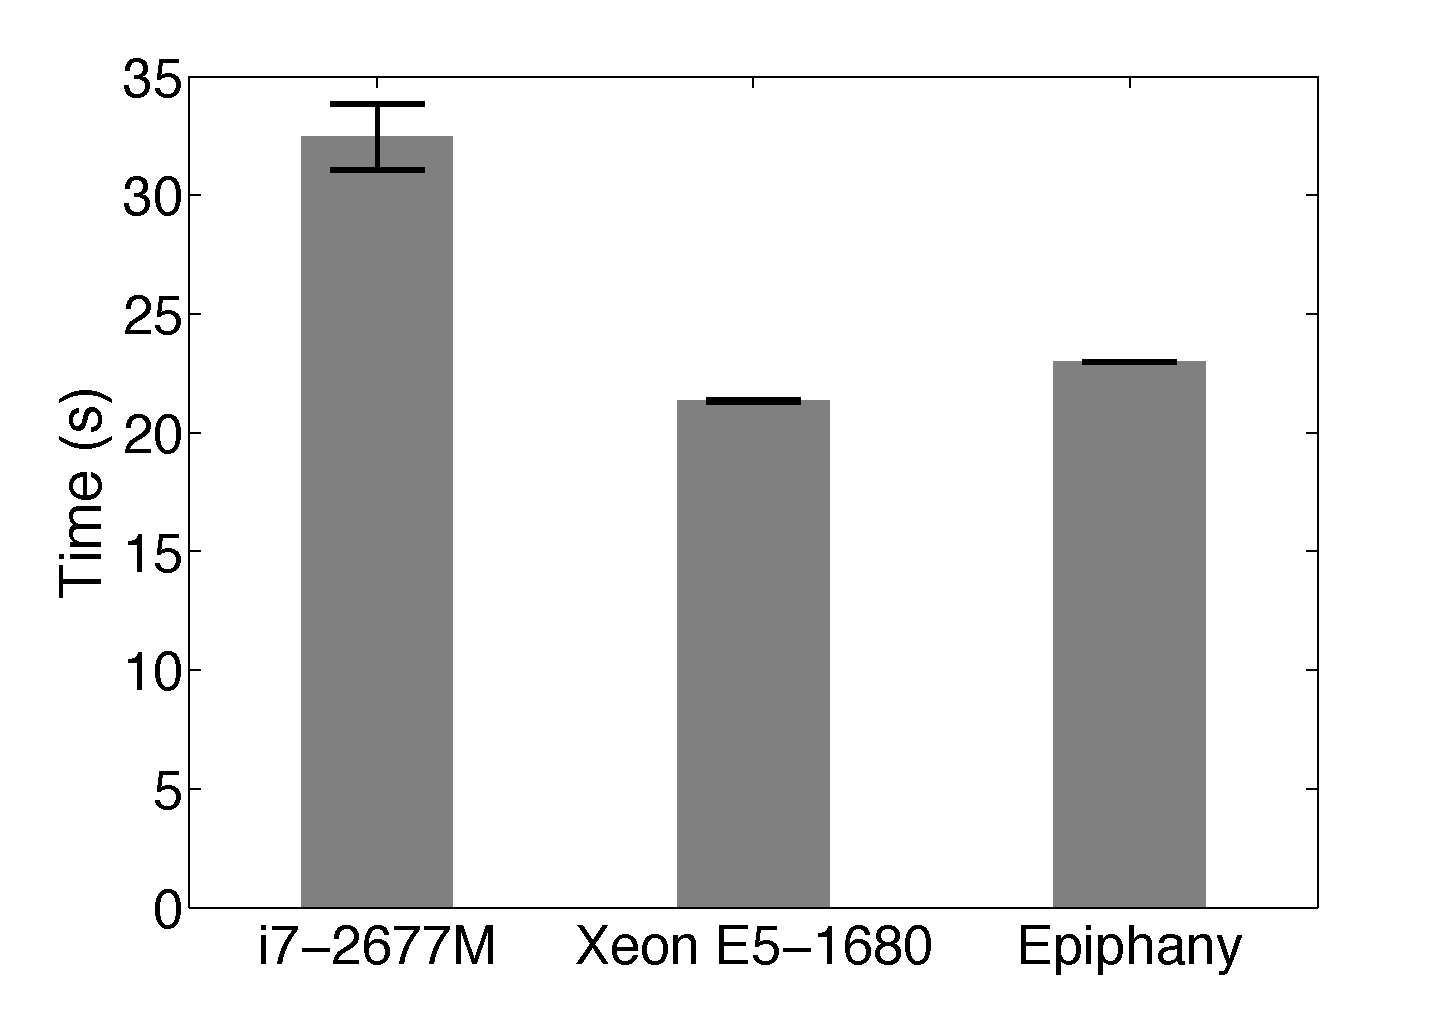
\includegraphics[width=\textwidth]{gt_1000.pdf}
	\caption{1000 records}
	\label{fig:k1000_comptime}
\end{subfigure}
\caption{Computation time for n\"{a}ive KNN search}
\label{fig:fullK256_1000}
\end{figure}